\RequirePackage{shellesc}
\immediate\write18{cd ..; tex braids_code.dtx}
\documentclass{article}

\usepackage{tikz}
\usetikzlibrary{braids}

\def\braidword{s_1 s_2^{-1} s_1^1 s_{1,4} s_{1-4} s_{4,1} s_{4-1}}

\begin{document}

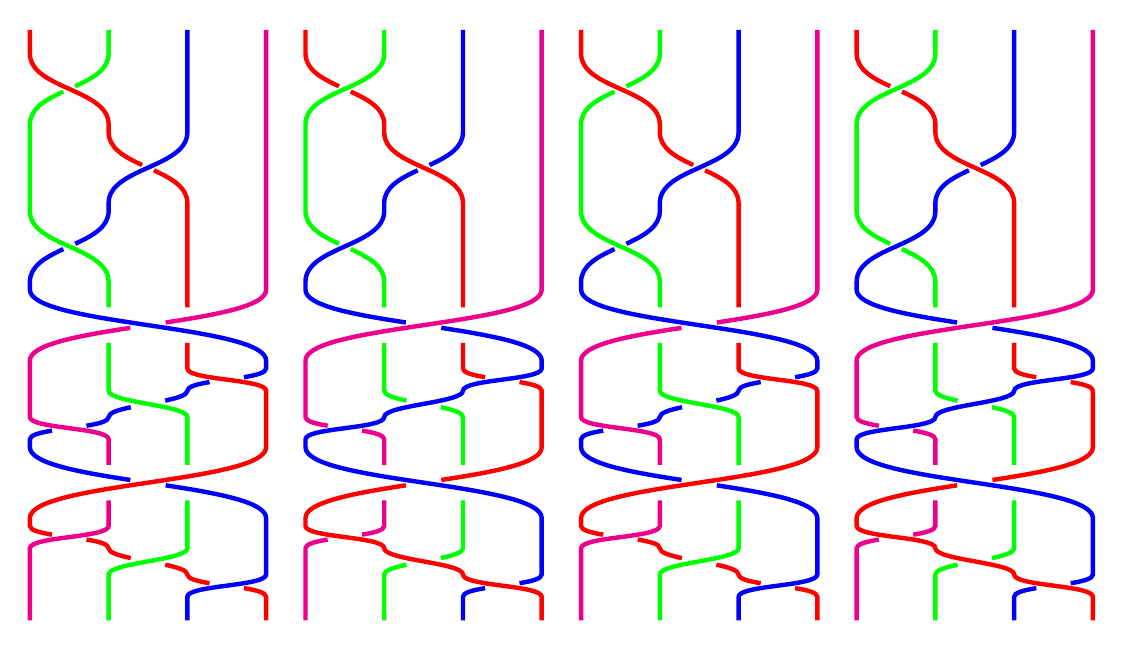
\begin{tikzpicture}[
  every braid/.style={
    braid/.cd,
    ultra thick,
    strand 1/.style={red},
    strand 2/.style={green},
    strand 3/.style={blue},
    strand 4/.style={magenta}
  }
]
\pic (braid) at (1,2) { braid/.expand once=\braidword };
\pic[
  braid/.cd,
  flip crossing convention,
] (braid) at (4.5,2) { braid/.expand once=\braidword };
\pic[
  braid/.cd,
  crossing convention=over,
] (braid) at (8,2) { braid/.expand once=\braidword };
\pic[
  braid/.cd,
  crossing convention=under,
] (braid) at (11.5,2) { braid/.expand once=\braidword };
\end{tikzpicture}

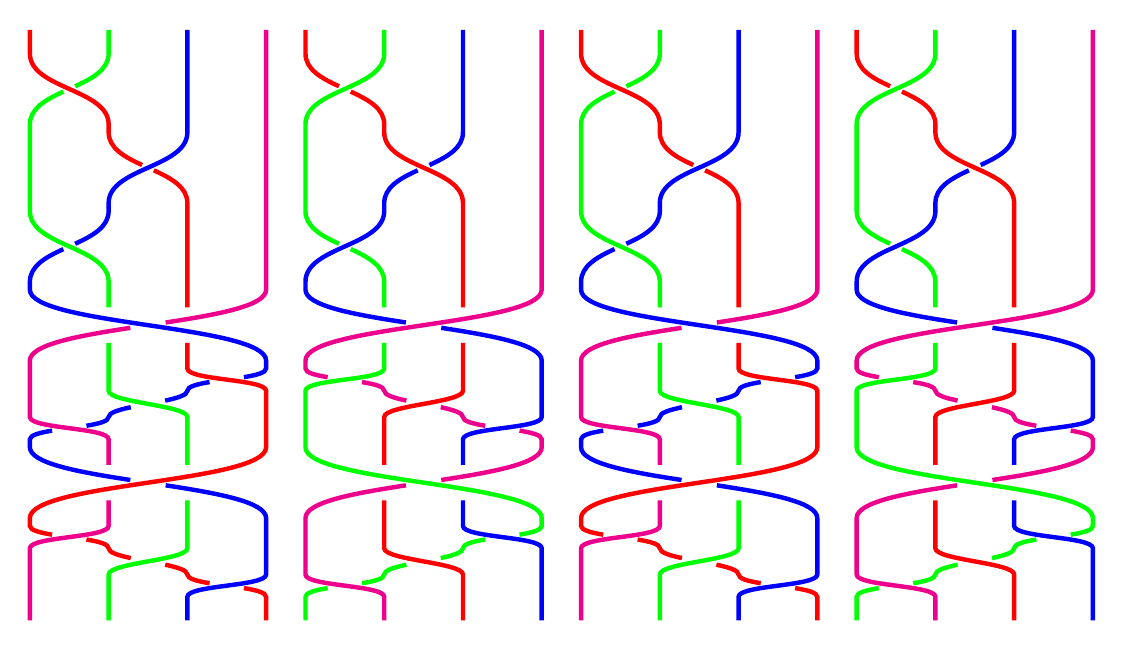
\begin{tikzpicture}[
  every braid/.style={
    braid/.cd,
    ultra thick,
    strand 1/.style={red},
    strand 2/.style={green},
    strand 3/.style={blue},
    strand 4/.style={magenta}
  }
]
\pic (braid) at (1,2) { braid/.expand once=\braidword };
\pic[
  braid/.cd,
  flip symbols,
] (braid) at (4.5,2) { braid/.expand once=\braidword };
\pic[
  braid/.cd,
  set symbols=over,
] (braid) at (8,2) { braid/.expand once=\braidword };
\pic[
  braid/.cd,
  set symbols=under,
] (braid) at (11.5,2) { braid/.expand once=\braidword };
\end{tikzpicture}

\end{document}
